\documentclass{article}
\usepackage[utf8]{inputenc}
\usepackage{amsmath}
\usepackage{graphicx}
\usepackage{float}


\graphicspath {}


\title{Networks and Random Processes Assignment 2}
\author{Charlie Pilgrim - 1864704}
\date{October 2018}

\begin{document}

\maketitle


\section{Kingman's Coalescent}

\subsection{A}

$N_t$ is the number of particles at time t with $N_0=L$. The process $(N_t : t \geq 0)$ has the state space $\{1,...,L\}$

\subsubsection{Transition Rate of the process}

$$r(n,n-1) = {L\choose 2} \, , \, n \geq 2$$

QUESTION - WHAT ABOUT SAME STATE?
$r(n,n) = $

QUESTION - WHAT ABOUT OTHER STATES - HOW TO WRITE IT?
$r(n, y) = \, , \, y \neq n,n-1$

\subsubsection{Generator}

This is a jump process, so the generator is

$$(\mathcal{L}f)(x) = \int_{\Re} r(x,y)[f(y)-f(x)]dy$$

For this process

$$(\mathcal{L}f)(n) = r(n,n-1)(f(n-1)-f(n))$$

$$(\mathcal{L}f)(n) = {n\choose 2} (f(n-1)-f(n))$$

\subsubsection{Master Equation}

The master equation is

$$\frac{d}{dt} \pi_t(n) = \pi_t(n+1)r(n+1,n) - \pi_t(n)r(n,n-1)$$

$$\frac{d}{dt} \pi_t(n) = \pi_t(n+1){n+1\choose 2} - \pi_t(n) {n \choose 2}$$

QUESTION - IS THIS RIGHT?
QUESTION - IS THE NOTATION OKAY?
QUESTION - WHAT ABOUT EDGES? 


\subsubsection{Ergodicity}

The process is ergodic.

\subsubsection{Absorbing States}

The unique absorbing state is $N = 1$.

\subsubsection{Stationary Distributions}

Let a distribution $\pi = [N=1, N=2,... ,N=L]$

The unique stationary distribution is 

$$\pi_0 = [1,0,...,0]$$

\subsection{B - Mean Time to Asorption}

The rate of coalescence, ie moving to the next state, for each state is

$$\lambda_n = r(n,n-1) = {n\choose 2} = \frac{n(n-1)}{2}$$

The times in each state are expnentially dsitributed as

$$f_t(n) = {n \choose 2} e^{-{n \choose 2}t}$$

The expected time in each state, or the waiting time, is given by 

$$\beta_n = \dfrac{1}{\lambda_n} = \frac{2}{n(n-1)}$$

The expected time to absorption is the sum of the expected waiting times in each of the states

$$E(T) = \sum_{n=2}^L\frac{2}{n(n-1)}$$

Bringing the 2 outside of the summand and splitting up into partial fractions

$$E(T) = 2\sum_{n=2}^L\frac{1}{n-1} - \frac{1}{n}$$


$$E(T) = 2(\frac{1}{1}-\frac{1}{2}+\frac{1}{2}-\frac{1}{3} + \frac{1}{3} + ... - \frac{1}{L-1} + \frac{1}{L+1} - \frac{1}{L})$$

All but the first and last terms cancel giving

$$E(T) = 2(1 - \frac{1}{L})$$


\subsection{C - Rescaled process}

Rescale the process to $N_t/L$

$$(\mathcal{L}^Lf)(n/L) = \frac{1}{L} {n\choose2} (f(\frac{n-1}{L}) - f(\frac{n}{L}))$$

Taylor expand and let $x=\frac{n}{L}$:

$$(\mathcal{L}^Lf)(x) = \frac{1}{L}\frac{n(n-1)}{2} (f(x) - \frac{1}{L}f'(x) + \frac{1}{L^2}f''(x) + O(\frac{1}{L^3}) - f(x))$$

Cancel terms, substitute $n=Lx$ and rearrange

$$(\mathcal{L}^Lf)(x) = (\frac{x^2}{2} - \frac{x}{2L})(- f'(x) + \frac{1}{L}f''(x) + O(\frac{1}{L^2}))$$

$$\lim_{L \to \infty} (\mathcal{L}^Lf)(x) = \frac{-x^2}{2}f'(x)$$

The state space goes from $\frac{1}{L}$ to $\frac{L}{L}$. As $L \to \infty$, this is $(0,1]$. 

The initial condition is $X_0 = \frac{L}{L} = 1$, 


\subsubsection{Deterministic}

The generator has no diffusion term, only drift. So there is no variance in the process and it must be entireley deterministic. 

\subsubsection{Computing $X_t$}

$$\frac{d}{dt}E(X_t) = E(-\frac{X_t^2}{2})$$

$X_t$ is deterministic, so

$$\frac{d}{dt}X_t = -\frac{X_t^2}{2}$$

$$\frac{dX_t}{X_t^2} = -\frac{1}{2}dt$$


$$\frac{1}{X_t} = \frac{1}{2}t + c$$


$$X_t = \frac{1}{\frac{t}{2}+c}$$

From the initial conditions, $X_0=1$, $c=1$.

$$X_t = \frac{1}{\frac{t}{2}+1}$$

\subsubsection{Comparing to result from b}

The result from part b was

$$E(T) = 2(1 - {1}{T})$$

For the rescaled process:

$$X_t = \frac{1}{\frac{t}{2}+1}$$

Consider when it reaches the absorbing state, i.e. $X_t = \frac{1}{L}$:

$$\frac{1}{L} = \frac{1}{\frac{t}{2}+1}$$

$$ L = \frac{t}{2}+1$$

$$ t = 2L(1-\frac{1}{L})$$


This is the same as the result from part b with a factor of L. This arises because we slowed down time by a factor of L during the rescaling process. 



\subsection{D - Simulation}

\begin{figure}[H]
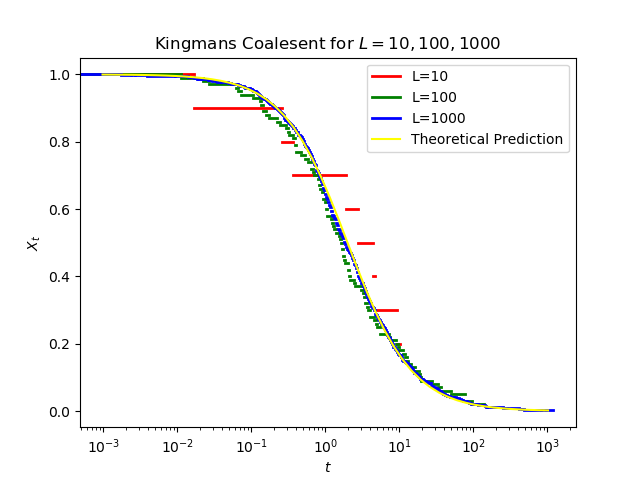
\includegraphics[scale=0.8]{kingsman_a.png} 
\caption{The Kingsman's coalescent rescaled process simulated for L=10, L=100, L=1000. The theoretical prediction of $X_t = \frac{1}{\frac{t}{2} + 1}$ is also shown.}
\label{fig:kingsman}
\end{figure}

Figure \ref{fig:kingsman} shows sample paths of the rescaled Kingsman's coalescent process for L=10,100 and 1000. The theoretical prediction for $L \to \infty$ is also shown. The simulations line up very well with the theoretical prediction.


\section{Ornstein-Uhlenbeck process}

\subsection{A}

The mean:

$$\frac{dm}{dt} = \frac{d}{dt}E(X_t) = E(-\alpha X_t) = -\alpha E(X_t)$$

$$\frac{dm}{dt} = -\alpha m(t)$$

$X_t^2$:

$$\frac{d}{dt}E(X_t^2) = E(- \alpha 2X_t^2 + \sigma^2)$$

$$\frac{d}{dt}E(X_t^2) = -2 \alpha E(X_t^2) + \sigma^2$$

The variance:

$$v(t) = E(X_t^2) -m(t)^2$$

$$\frac{dv}{dt} = \frac{d}{dt}E(X_t^2) - 2m\frac{dm}{dt}$$

$$\frac{dv}{dt} = -2 \alpha E(X_t^2) + \sigma^2 + 2 \alpha m^2$$

\subsection{B}

\subsubsection{Solution of $m(t)$}

Solving for m(t), and considering the initial conditions, $c=x_0$

$$m(t) = x_0 e^{-\alpha t}$$

\subsubsection{Solution of $v(t)$}

Solving for v(t)

$$\frac{dv}{dt} = -2 \alpha (v + m^2) + \sigma^2 + 2 \alpha m^2$$

$$\frac{dv}{dt} +  2 \alpha v = \sigma^2$$

Homogenous solution:

$$v_hom = c_2 e^{-2 \alpha t}$$

Particular solution:

$$v_part = \frac{\sigma^2}{2 \alpha}$$

Full solution:

$$ v(t) = c_2 e^{-2 \alpha t} + \frac{\sigma^2}{2 \alpha}$$

From initial conditions, $v(0) = 0$:

$$ v(t) = \frac{\sigma^2}{2 \alpha}(1-e^{-2 \alpha t})$$

\subsubsection{Distribution}

As a Gaussian process, the distribution is fully described by the mean and variance.

$$f(X_t) = \dfrac{1}{\sqrt{\frac{2 \pi \sigma^2 (1-e^{-2 \alpha t})}{2 \alpha}}}exp(\frac{- \alpha (x - x_0 e^{- \alpha t})^2}{\sigma^2 (1-e^{-2 \alpha t})}$$

IS THAT RIGHT?

\subsubsection{Stationary Distribution}

Given enough time, the process will converge to a Gaussian stationary distribution.  

$$\lim_{t \to \infty} m(t) = 0$$

$$\lim_{t \to \infty} v(t) = \frac{\sigma^2}{2 \alpha}$$

The stationary distribution is $\sim N(0,\frac{\sigma^2}{2 \alpha})$ 

$$f_0(X_t) = \dfrac{1}{\sqrt{\frac{\pi \sigma^2}{\alpha}}}exp(\frac{- \alpha x^2}{\sigma^2})$$

\subsection{Simulation}

\begin{figure}[H]
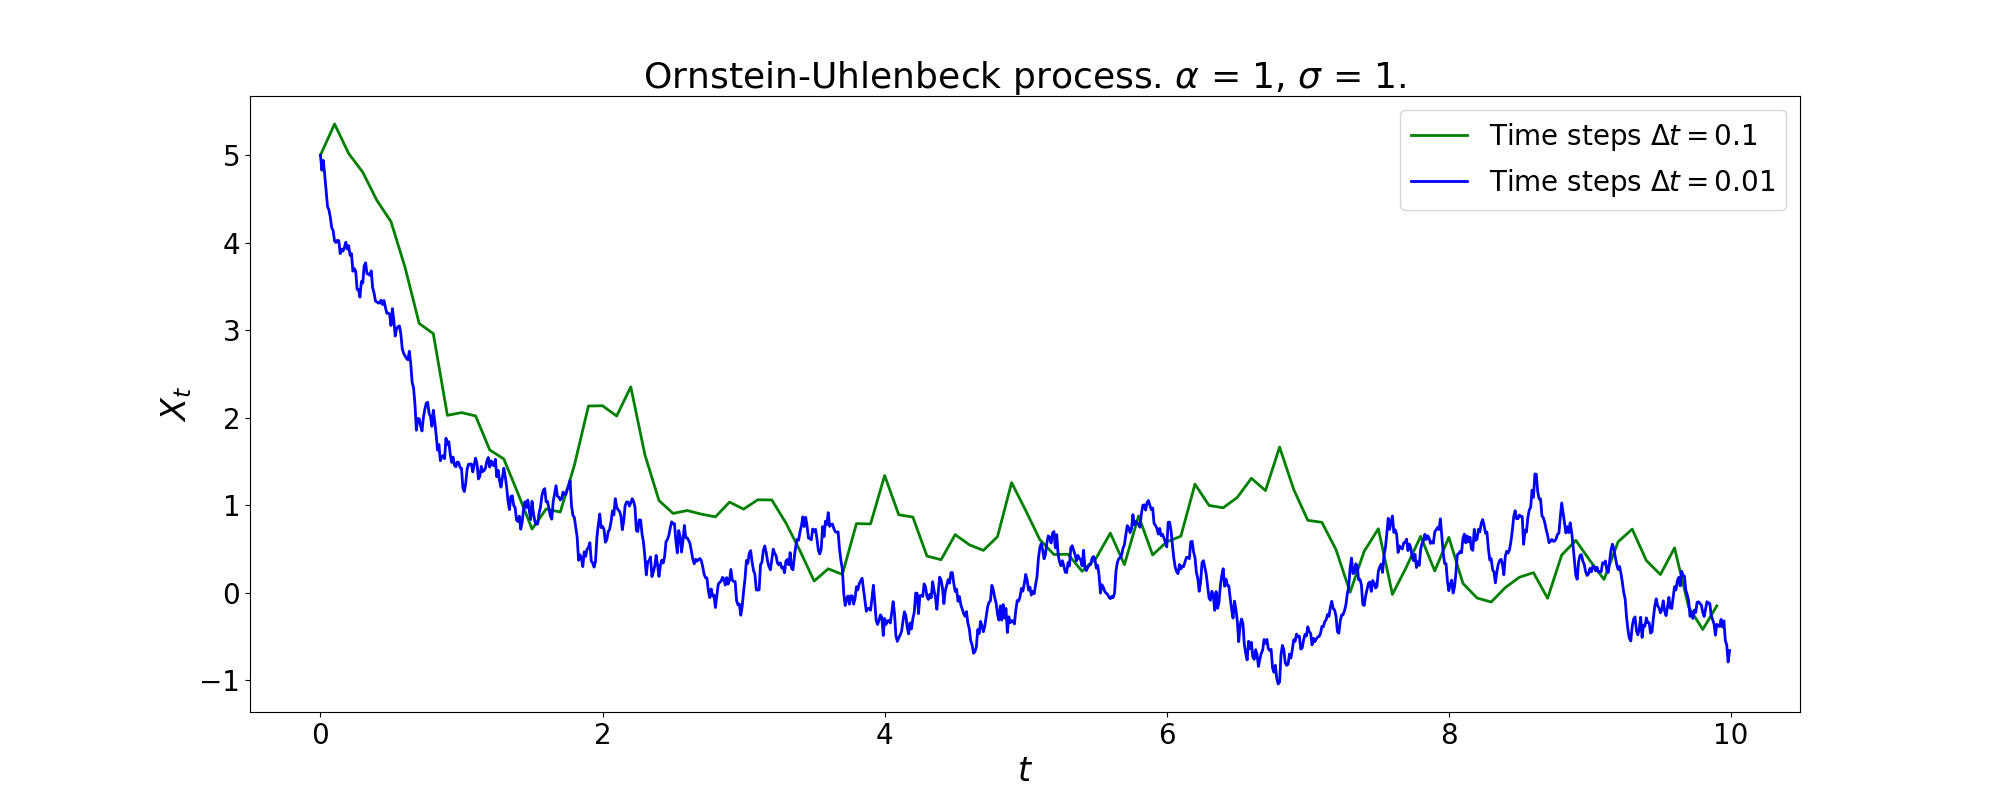
\includegraphics[scale=0.25]{ou_process_a.png} 
\caption{The Ornstein-Uhlenbeck process with $\alpha=1$, $\sigma^2=1$ and $X_0 = 5$. Simulated for 10 seconds with timsteps $\Delta t =0.1$ and $0.01$}
\label{fig:ou_process}
\end{figure}

Figure \ref{fig:ou_process} shows the Ornstein-Uhlenbeck process simulated. The process begins at $X_0=5$, and expereinces a "force" pulling it towards zero. As time progresses, the process moves towards $X_t=0$ and the noise term begins to dominate the behaviour. Both choices of timestep give a similar result.

\section{Moran Model and Wright-Fisher diffusion}

\subsection{A}

\subsubsection{State space}

Let the total possible L types be 

$$T = \{1,2,...,L\}$$

Each of the L individuals can have any of those types, so the state space is 

$$S = \{1,2,3,...,L\}^L$$

\subsubsection{Irreducibility}

It is not irreducible because there are absorbing states. 

\subsubsection{Stationary distributions}

The absorbing states are where all individuals have the same type

$$x_k = [k,k,...,k] \quad \forall k \in \{1,2,...,L\}  $$

The stationary distributions are any linear combination of the absorbing states that sum to 1. 

$$\pi(y) = \sum_{k=1}^L \alpha_k \pi_k(y)$$

$$\sum_{k=1}^L \alpha_k = 1$$

The coefficients, $\alpha_k$, are determined by the initial conditions and can be thought of as the probability of each type "winning" and taking over all individuals. 

\subsection{B}

\subsubsection{Markov process}

$N_t : t \geq 0$ is a Markov process. It's future distribution is determined only by it's current state, not the specific history.

\subsubsection{State space}

Each type can have any integer between 0 and L types, and there are L types, so the state space is 

$$S = \{0,1,2,...,L\}^L$$

\subsubsection{Generator}

For each type, we assume that the number of individuals of that type, $n$, can only increase and decrease by 1 at one moment in time, i.e only one event happens at a time. The rates of gain and loss can be described as:

$$r(n,n+1) = \frac{n(L-n)}{L-1}$$

$$r(n,n-1) = \frac{n(L-n)}{L-1}$$

These are symmetrical. 


This is a jump process, so the generator is

$$(\mathcal{L}f)(x) = \int_{\Re} r(x,y)[f(y)-f(x)]dy$$

For this process

$$(\mathcal{L}f)(n) = r(n,n-1)(f(n-1)-f(n)) + r(n,n+1)(f(n+1)-f(n))$$

$$(\mathcal{L}f)(n) = \frac{(L-n)n}{L-1}(f(n-1) + f(n+1) - 2f(n))$$




\subsubsection{Irreducibility}

The process is not irreducible because there are absorbing states. 

\subsubsection{Stationary dsitributions}

The absorbing states are where one type has $N_k = L$ and the rest $N_k=0$. i.e

$$ \pi_k(y) = \delta_{y,k} = \begin{cases}
L \quad , \quad y=k\\
0 \quad , \quad \text{otherwise}\\
\end{cases}$$

?? IS THAT RIGHT? 
 
\subsubsection{Limiting distribution}

As $t \to \infty$ with initial condition $N_0 = 1$. By symmetry each type has the same chance of "winning", therefore the limiting distribution is

$$ \pi_{\infty} = [\frac{L-1}{L},0,0,...,0,\frac{1}{L}]$$

\subsection{C}

\subsubsection{$m_1(t)$}

$$\frac{d}{dt}(E(N_t)) = E(\frac{n(L+n)}{L-1}(n + 1 + n - 1 -2n)$$

$$\frac{d}{dt}(E(N_t)) = 0$$

$N_0 = n$, therefore $E(N_t)=n$.

\subsubsection{$m_2(t)$}

$$\frac{d}{dt}(E(N^2)) = E(\frac{n(L+n)}{L-1}((n + 1)^2 + (n - 1)^2 -2n^2)$$

$$\frac{d}{dt}(E(N^2)) = E(\frac{n(L+n)}{L-1}(n^2 + 2n + 1 + n^2 - 2n + 1 -2n^2)$$

$$\frac{d}{dt}(E(N^2)) = E(\frac{2n(L+n)}{L-1})$$

$$\frac{d}{dt}(E(N^2)) = \frac{2L}{L-1}n + \frac{2}{L-1}E(N^2)$$

Solution in the form:

$$E(N^2) = Ae^{\frac{-2t}{L-1}} + B$$

From initial condition, $A=N_0^2$

Substitute everything into the original differential equation:

$$\frac{-2n}{L-1}e^{\frac{-2t}{L-1}} = \frac{2Ln}{L-1} + \frac{2}{L-1}e^{\frac{-2t}{L-1}} + \frac{2B}{L-1}$$

$$B = Ln(1-e^{\frac{-2t}{L-1}})$$

$$E(N^2) = n^2e^{\frac{-2t}{L-1}} + Ln(1-e^{\frac{-2t}{L-1}})$$


\subsubsection{Absorption probabilities}

By symmetry, each individual has an equal chance of winning. So the absorption probabilities are

$$p(L) = \frac{n}{L}$$

$$p(0) = 1 - \frac{n}{L}$$



\subsubsection{Absorption time scales with system size L}

The expected value of $E(N_t)=n$.

The variance is given by 

$$Var(N_t) = n^2e^{\frac{-2t}{L-1}} + Ln(1-ne^{\frac{-2t}{L-1}}) - n^2$$

$$Var(N_t) = (Ln - n^2)(1- e^{\frac{-2t}{L-1}})$$

The standard deviation grows with time. As the standard deviation grows, it becomes more and more likely that the process will be absorbed. 

Let $x = \frac{n}{L}$

$$Var(N_t) = L^2 (x -x^2)(1- e^{\frac{-2t}{L-1}})$$

$$\sigma(N_t) = L (x -x^2)^{\frac{1}{2}}(1- e^{\frac{-2t}{L-1}})^{\frac{1}{2}}$$

$$\frac{\sigma(N_t)}{L} = (x -x^2)^{\frac{1}{2}}(1- e^{\frac{-2t}{L-1}})^{\frac{1}{2}}$$

The ratio $\frac{\sigma}{L}$ can be thought of as a proxy for the absorption probability. For different L, equal values of $\frac{\sigma}{L}$ will have very similar absorption probability distributions in x. 

If we were to increase L while fixing $\frac{\sigma}{L}$, i.e. fixing the absoprtion probability, then the time would scale linearly with L. From this argument, we can see that absorption time will scale linearly with L.  


\subsection{D}

\subsubsection{Rescaling limit}

$$(\mathcal{L}f)(n) = \frac{(L-n)n}{L-1}(f(n+1) + f(n-1) - 2f(n))$$

Rescale by dividing state space by L, multiplying time by $L^\alpha$ and changing the variable to $x=\frac{n}{L}$:

$$(\mathcal{L}f)(x) = \frac{(L-xL)xL}{L-1}L^\alpha(f(x+\frac{1}{L}) + f(x+\frac{1}{L}) - 2f(x))$$

Taylor expand and simplify:

$$(\mathcal{L}f)(x) = \frac{(L-xL)xL}{L-1}L^\alpha(\frac{1}{L^2}f''(x) - O(\frac{1}{L^3})$$

$$(\mathcal{L}f)(x) = \frac{L^\alpha}{L} \frac{xL^2 - x^2L^2}{1-\frac{1}{L}}(\frac{1}{L^2}f''(x) - O(\frac{1}{L^3})$$

Set $\alpha=1$ to get a non-trivial scaliming limit:

$$(\mathcal{L}f)(x) = (\frac{x - x^2}{1-\frac{1}{L}})f''(x) - O(\frac{1}{L})$$

Take limit $L \to \infty$:

$$(\mathcal{L}^Lf)(x) = \lim_{L \to \infty} (\mathcal{L}f)(x) = (x - x^2)f''(x)$$

$$(\mathcal{L}^Lf)(x) = x(1 - x)f''(x)$$

\subsubsection{Fokker-Planck Equation}

$$\frac{\partial}{\partial t}p_t(x,y) = \frac{\partial^2}{\partial y^2} (y(1-y) p_t(x,y)$$

WHAT DOES THIS MEAN?

\subsection{E}

\subsubsection{$m(t)$}

$$\frac{d}{dt}E(M) = 0$$

No change in $E(M_t)$ with time. Let $E(M_t) = M_0$

\subsubsection{$v(t)$}

$$\frac{d}{dt}E(M^2) = E(2M - 2M^2)$$

$$\frac{d}{dt}E(M^2) = 2M_0 - 2E(M^2)$$

This is a differential equations. Homogenous solution:

$$E(M^2)_{hom} = c e^{-2t}$$

$$E(M^2)_{part} = M_0$$

Full solution:

$$E(M^2) = c e^{-2t} + M_0$$

The initial conditions are $M(0)^2 = M_0^2$ 

$$E(M^2) = (M_0^2 -M_0)e^{-2t} + M_0$$

The variance:

$$v(t) = E(M^2) - E(M)^2$$

$$v(t) = (M_0^2 -M_0)e^{-2t} + M_0 - M_0^2$$

Factorises to:

$$v(t) = M_0(1-M_0)(1-e^{-2t})$$

It is not Gaussian because it has a limited state space, Gaussians go to infinity.

\subsection{F - Simulation}

\begin{figure}[H]
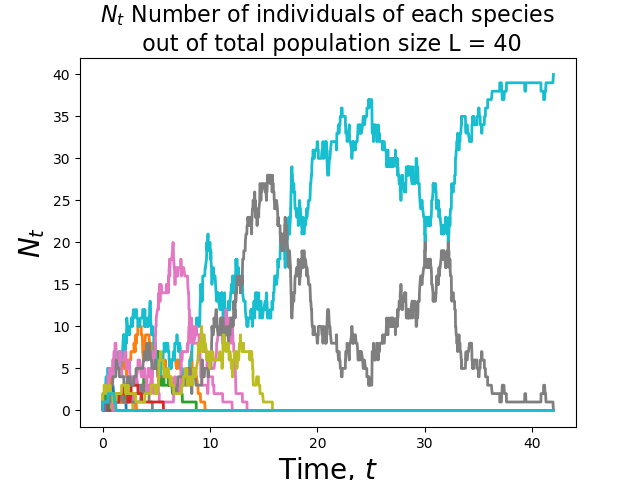
\includegraphics[scale=0.8]{moran_a.png} 
\caption{The Moran model process simulated for a population of L=40. $N_t$ is the number of individuals of each type, plotted against continuous time.} 
\label{fig:moran}
\end{figure}

Figure \ref{fig:moran} shows a simulation of the Moran model process. The number of each individuals of each type is shown a a function of continuous time. Gains in one type must conincide with losses of another type, as they must always sum to 40. This can be seen in the symmetry in the patterns between the two surviving types after around $t=18$.

\section{Barabasi-Albert}

\subsection{Tail of degree distribution}

\begin{figure}[H]
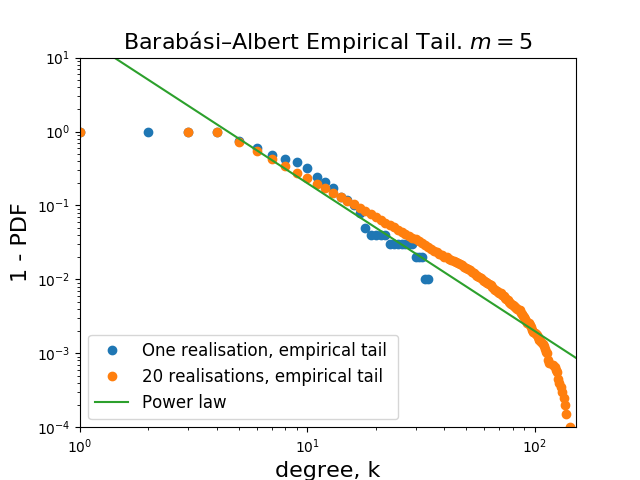
\includegraphics[scale=0.8]{barabasi_a.png} 
\caption{The Barabasi-Albert preferential attachment model simulated starting with 5 nodes and each new node attaching to 5 existing nodes. N = 1000 nodes. 1 - Probability Density Function is shown, estimated empircally for 1 realisation and 20 realisations. The tail fits closely to a power law with $\alpha=-2$.} 
\label{fig:barabasi}
\end{figure}

Figure \ref{fig:barabasi} shows a simulation of the Barabasi-Albert model. The emprical tail fits closely to a power law with $\alpha = -2$.

\subsection{Distribution of degree of nearest neighbour}

\begin{figure}[H]
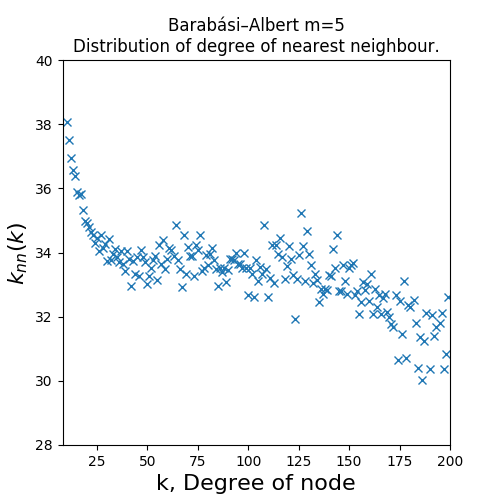
\includegraphics[scale=0.8]{degree_neighbour_a.png} 
\caption{The degree distribution of nearest neighbours for Barabasi-Albert model averaged over 100 realisations with $m=5$, $N = 1000$.} 
\label{fig:neighbour}
\end{figure}

Figure \ref{fig:neighbour} shows the expected degree of the nearest neightbour for the Barabasi-Albert simluation with 100 realisations. There is not a strong correlation between a node's degree and the expected degree of their nearest neighbour. The graphs typically appear to be uncorrelated.


\section{Erdos-Enyi Random Graph}

\subsection{Component sizes}

\begin{figure}[H]
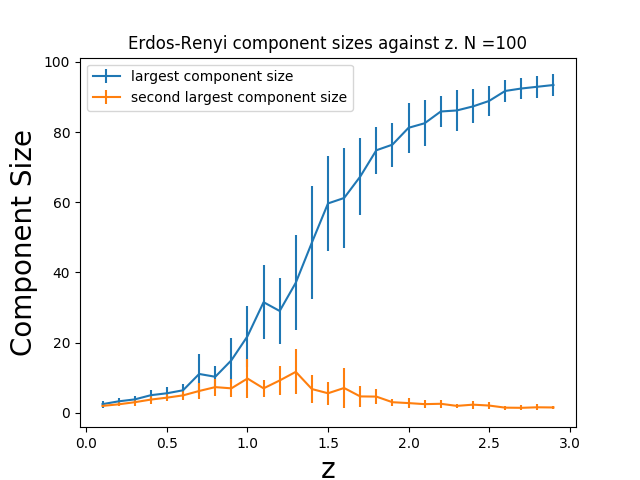
\includegraphics[scale=0.8]{erdos_a.png} 
\caption{First and sexond largest component sizes for Erdos-Renyi random graphs as a function of z, the average degree of each node. $N=100$} 
\label{fig:erdos_100}
\end{figure}


\begin{figure}[H]
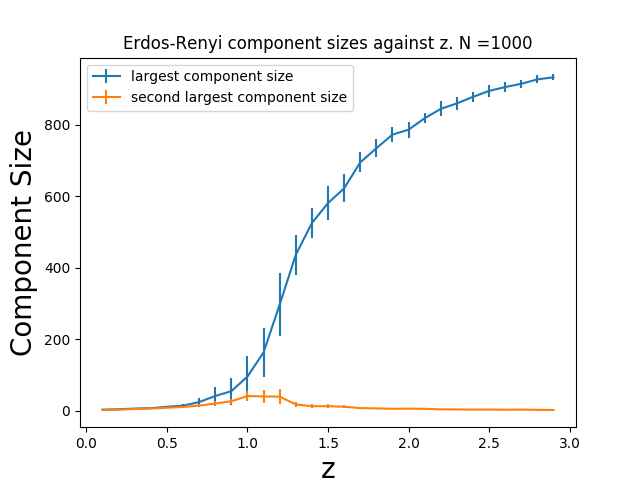
\includegraphics[scale=0.8]{erdos_1000_a.png} 
\caption{First and sexond largest component sizes for Erdos-Renyi random graphs as a function of z, the average degree of each node. $N=1000$} 
\label{fig:erdos_1000}
\end{figure}

Figures \ref{fig:erdos_100} and \ref{fig:erdos_1000} show the 2 largest component sizes for Erdos-Renyi random graphs as a function of z, for 20 realisations. At $z=1$, the system undergoes a phase transition, which can be seen more clearly in \ref{fig:erdos_1000}. 

Below $z=1$ there are many small components, and the sizes of the largest ones grow as $~O(logN)$. Above $z=1$ the largest components grow as $~O(N)$. At the boundary the size of the components are distributed by a scale free power law distribution.

\subsection{Clustering Coefficient}

\begin{figure}[H]
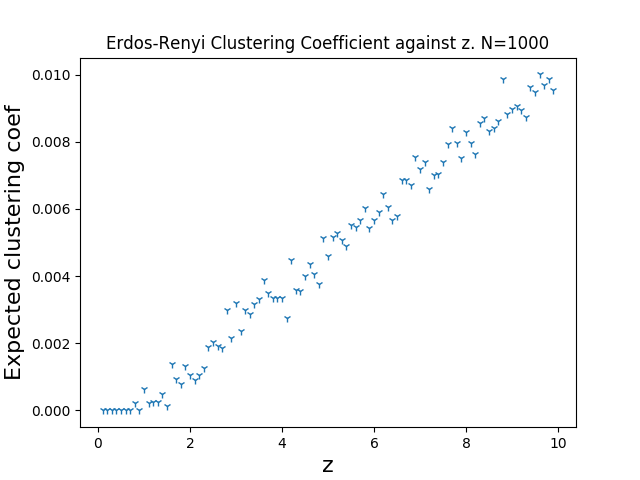
\includegraphics[scale=0.8]{clustering_a.png} 
\caption{Erdod-Renyi random graphs clustering coefficeint as a function of z for 10 realisations and total nodes N=1000.} 
\label{fig:clustering}
\end{figure}

Figures \ref{fig:clustering} shows the emprical clustering coefficients of Erdos-Renyi random graphs at a range of z values. There is a linear relationship between z and the expected clustering coefficient. Even at relatively high z, the clustering coefficient is low. 

\subsection{Degree Distribution}


\begin{figure}[H]
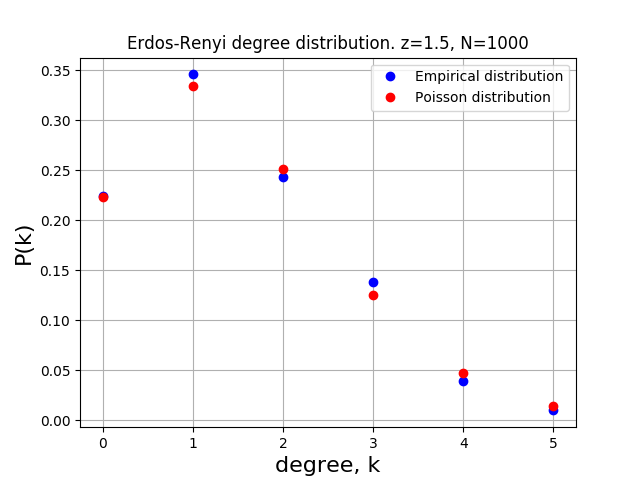
\includegraphics[scale=0.8]{poisson_a.png} 
\caption{Erdod-Renyi random graphs degree distribution, averaged over 20 realisations. And a Poisson distribution with $z=1.5$ as a shape parameter.} 
\label{fig:poisson}
\end{figure}

Figure \ref{fig:clustering} shows the average degree distibution for 20 realisations of Erdos-Renyi random graphs of size $N=1000$. The discrepancy between the empirical data and the Poisson distribution will reduce as N increases. In the limit as $N \to \infty$ the degree distribution should fit a Poisson distribution. 

\end{document}





